\section{Theoretical Analysis}
\label{sec:analysis}

In this section, the circuit $RC$ shown in Figure~\ref{fig:circuit} is analysed
theoretically.



%b = [Id; -Va/R1; Va/R1; Id]

\[
  \begin{bmatrix}
    - \frac{1}{R_1} & \frac{1}{R_1} + \frac{1}{R_2} + \frac{1}{R_3} & -\frac{1}{R_2} & -\frac{1}{R_3}                                & 0              & 0                              & 0             \\
    0               & K_b + \frac{1}{R_2}                           & -\frac{1}{R_3} & - K_b                                         & 0              & 0                              & 0             \\
    0               & 0                                             & 0              & 0                                             & 0              & -\frac{1}{R_6} - \frac{1}{R_7} & \frac{1}{R_7} \\
    0               & K_b                                           & 0              & -K_b - \frac{1}{R_5}                          & \frac{1}{R_5}  & 0                              & 0             \\
    0               & -\frac{1}{R_3}                                & 0              & \frac{1}{R_3} + \frac{1}{R_4} + \frac{1}{R_5} & -\frac{1}{R_5} & -\frac{1}{R_7}                 & \frac{1}{R_7} \\
    0               & 0                                             & 0              & 1                                             & 0              & \frac{K_d}{R_6}                & -1            \\
    1               & 0                                             & 0              & 0                                             & 0              & 0                              & 0             \\
  \end{bmatrix}
  \begin{bmatrix}
    V_1 \\ V_2  \\ V_3 \\ V_5 \\ V_6 \\ V_7 \\ V_8
  \end{bmatrix}
  =
  \begin{bmatrix}
    0 \\ 0 \\ 0 \\ 0 \\ 0  \\ 0 \\ V_s
  \end{bmatrix}
\]

\hfill

% \begin{table}
%   \parbox{.45\linewidth}{
%     \centering
%     \begin{tabular}{|c|c|}
%       \hline
%       {\bf Name} & {\bf Value [A or V]} \\ \hline
%       \input{op_nodal1_tab}
%     \end{tabular}
%     \label{tab:op_tabNodalTeo1}
%     \caption{Results of Nodal Analysis of the circuit for t < 0. A variable that begins  with \textit{I} names a \textit{current} in \textit{Ampere}; the ones that start with \textit{V} name a \textit{voltage} in \textit{Volt}}
%   }
%   \hfill
%   \parbox{.45\linewidth}{
%     \centering
%     \begin{tabular}{|c|c|}
%       {\bf Name} & {\bf Value [A or V]} \\ \hline
%       @gib[i] & -2.65517e-04\\ \hline
@id[current] & 1.025904e-03\\ \hline
@r1[i] & -2.53670e-04\\ \hline
@r2[i] & -2.65517e-04\\ \hline
@r3[i] & -1.18476e-05\\ \hline
@r4[i] & 1.220737e-03\\ \hline
@r5[i] & -1.29142e-03\\ \hline
@r6[i] & 9.670671e-04\\ \hline
@r7[i] & 9.670671e-04\\ \hline
v(1) & -7.95657e+00\\ \hline
v(2) & 3.950179e+00\\ \hline
v(3) & -3.64391e-02\\ \hline
v(4) & -4.95541e+00\\ \hline
v(5) & -6.94792e+00\\ \hline
v(6) & -5.78231e-01\\ \hline
v(7) & 2.284139e-01\\ \hline
v(8) & -4.95541e+00\\ \hline

%       \hline
%     \end{tabular}
%     \label{tab:op_tabNodalSpice1}
%     \caption{Table with results from Ngspice to find out the voltages and currents in each node and branch. A variable that begins  with \textit{I} names a \textit{current} in \textit{Ampere}; the ones that start with \textit{V} name a \textit{voltage} in \textit{Volt} }
%   }
% \end{table}



By solving these equations with a script of \textit{Octave}, we got the following results presented in table \ref{tab:op_tabReqTeo}.


By looking at first glance, the results do not seem right. In order to try and get a better understading of what was going on, we used an alternative method to find the equivalent resistance: we replace the capacitor with an indepedent voltage source of $1 A$ in order to do the calculation of the equivalent resistance easier.
We run mesh analysis in the circuit with the elementar currents shown in \ref{fig:circuit}. The results are shown in the following system of equations:


As can be easily seen, the first three equations are linearly independent of each other and the last equations is disconnect from the other ones. So, $I_2 = I_3 = I_4 = 0$. As result, from the last equation, we know that
the equivalent resistance is equal to $R_5$.


From the previous calculations, we have as forced solution in $v_6$:

\begin{equation}
  v_{6f} = \Re (\tilde{V_6} e^{j 2\pi f t}) = 0.5809432*cos(2 \pi f t - 1.718634)
  \label{forcedSolution}
\end{equation}



\subsection{Frequency response}

In order to evaluate the frequency response of the circuit in the asked nodes, we have to find a way of evaluating the following equation:


\[
  \begin{bmatrix}
    \frac{1}{R1} + \frac{1}{ZC1} + \frac{1}{ZC2} & -\frac{1}{ZC2} \\
    -\frac{1}{ZC1}                               & -\frac{1}{R2}  \\
  \end{bmatrix}
  \begin{bmatrix}
    VIN \\ VOUT
  \end{bmatrix}
  =
  \begin{bmatrix}
    \frac{VIN}{R1} \\ 0
  \end{bmatrix}
\]

\hfill


\begin{equation}
  T(\omega) = \frac{\widetilde{V_{out}}}{\widetilde{V_{in}}}
  \label{frequencyR}
\end{equation}

where in function \ref{frequencyR} we have $\widetilde{V_{out}} = \tilde{V_6}$ and $\widetilde{V_{out}} = \tilde{V_c}$ as been asked.

Because of the difficulty in solving the system of equation found in the section of \textit{Forced Solution} to arrange the function \ref{frequencyR} explicitly, we find out the solution numerically using Octave.

In plot \ref{fig:argT}, we have the phase, obtained by taking the $arg(T(\omega))$, as function of $log(\omega)$ for the range of $0.1Hz$ to $1MHz$.

\begin{figure}[h] \centering
  \includegraphics[width=1.\linewidth]{gain.eps}
  \caption{Graph of the magnitude of the gain (dB) as a function of log(f) in Hz}
  \label{fig:absT}
\end{figure}

In plot \ref{fig:absT} we have the magnitude, calculated from $20*log_{10}(abs(T(\omega)))$ as function of $log(\omega)$ for the same range of frequencies as given before.

\begin{figure}[h] \centering
  \includegraphics[width=1.\linewidth]{phase.eps}
  \caption{Graph of the phase  of T($\omega$) as function of log(f) }
  \label{fig:argT}
\end{figure}


\begin{table}
  \parbox{.45\linewidth}{
    \centering
    \begin{tabular}{|c|c|c|}
      \hline
      $Z_{input}$ & -1.312927e-01\\ \hline
$Z_{output}$ & 0.000000e+00\\ \hline
Max $Gain_{dB}$ & 1.835867e+01\\ \hline
Central frequency [Hz] & 9.660509e+02\\ \hline

    \end{tabular}
    \label{tab:TheoreticalResults}
    \caption{Theoretical Results of Nodal Analysis of the circuit used to determine the equivalent resistance seen by the capacitor. A variable that begins  with \textit{I} names a \textit{current} in \textit{Ampere}; the ones that start with \textit{V} name a \textit{voltage} in \textit{Volt} }
  }
  \hfill
  %   \parbox{.45\linewidth}{
  %     \centering
  %     \begin{tabular}{|c|c|}
  %       {\bf Name} & {\bf Value [A or V]} \\ \hline
  %       \input{opb_tab}
  %       \hline
  %     \end{tabular}
  %     \label{tab:op_tabReqSpice}
  %     \caption{Ngspice results of Nodal Analysis of the circuit used to determine the equivalent resistance seen by the capacitor. A variable that begins  with \textit{I} names a \textit{current} in \textit{Ampere}; the ones that start with \textit{V} name a \textit{voltage} in \textit{Volt} }
  %   }
\end{table}


% As we can see, the phase and the magnitude of $T_{Vs}$ is constant as imposed by the source.
% From the plots of $T_{Vc}$, we see that the response of the capacitor for frequencies smaller than the frequency $f_c = \frac{1}{R_{eq}C} = 318.674 Hz$, the output voltage is almost equal to input voltage and that the signals have the same phase.
% For frequencies much bigger than $f_c$, the $V_{out} \rightarrow 0$, as seen  in \ref{fig:absT} and the signal is $-180$ degrees ou of phase.
% For frequencies in a near range of $f_c$, we have an abrupt decline in $V_{out}$ and phase.

% In regard to $T_{V6}$, we have that the magnitude of its transfer function dcreases to a constant value, magnitude of the phasor in $v_8$, which is expected due to the fact that the impedance fo the capacitor decreases in module as $\omega$ increases



% These differences are due to the fact that in $T_{V6}$ we see how the magnitude of the output voltage between node 0 and node 6(the output voltage has the influence of resistors too). While in
% $T_{Vc}$ we are seeing how the volatge across the capacitor changes with the frequency(acts as a low pass filter).